%-----------------------------------------------------------------------------
%
%               Template for sigplanconf LaTeX Class
%
% Name:         sigplanconf-template.tex
%
% Purpose:      A template for sigplanconf.cls, which is a LaTeX 2e class
%               file for SIGPLAN conference proceedings.
%
% Guide:        Refer to "Author's Guide to the ACM SIGPLAN Class,"
%               sigplanconf-guide.pdf
%
% Author:       Paul C. Anagnostopoulos
%               Windfall Software
%               978 371-2316
%               paul@windfall.com
%
% Created:      15 February 2005
%
%-----------------------------------------------------------------------------
\documentclass{sigplanconf}

% The following \documentclass options may be useful:

% preprint      Remove this option only once the paper is in final form.
% 10pt          To set in 10-point type instead of 9-point.
% 11pt          To set in 11-point type instead of 9-point.
% authoryear    To obtain author/year citation style instead of numeric.
\usepackage{amsmath}
\usepackage{amssymb}
\usepackage{amsthm}
\usepackage{graphicx}
\usepackage{listings}
\usepackage{color}
\usepackage[utf8]{inputenc}
\usepackage{ulem}
\usepackage{mathtools}
\usepackage{realboxes}

\usepackage{bussproofs}
%--------------------BNF----------------------------------------------
\usepackage{syntax}
\setlength{\grammarparsep}{10pt}
\setlength{\grammarindent}{9em}


%--------------------Langage LIDL----------------------------------------------
\definecolor{codebackground}{rgb}{0.95,0.95,0.95}
\definecolor{keywordcolor}{rgb}{0.1,0.1,0.5}
\definecolor{commentcolor}{rgb}{0.1,0.5,0.1}


\lstdefinelanguage{lidl}
{
 keywords={activation, boolean, number, text, in, out, type, interface, interaction, implementing, is  },
 sensitive=false,
 morecomment=[l]{//},
 morecomment=[s]{/*}{*/},
 morestring=[b]",
}

\lstset{
 language=lidl,
 basicstyle=\ttfamily,            % print whole listing small
 keywordstyle=\color{keywordcolor}\bf\ttfamily,% underlined bold black keywords
 tabsize=2,                    % sets default tabsize to 2 spaces
 captionpos =b                 % sets the caption-position to bottom
 keepspaces = true,             % keeps spaces in text
 % identifierstyle=,           % nothing happens
 commentstyle=\color{commentcolor}\textit,         % white comments
 stringstyle=\ttfamily,        % typewriter type for strings
 showstringspaces=false,       % no special string spaces
 %columns=flexible,             % colonnes "flexibles"
 basewidth={0.5em},           % dimension des colonnes
 fontadjust=true,              % pour ajuster les polices
 breaklines=true ,             % pour le retour à la ligne dans les colonnes
% backgroundcolor=\color[rgb]{0.95,0.95,0.95}
  backgroundcolor=\color{codebackground}
}

\newcommand{\code}[1]{\Colorbox{codebackground}{\lstinline{#1}}}

\newcommand{\codemath}[1]{\colorbox{codebackground}{$\mathtt{\displaystyle #1}$}}
%---------------------------------------------------------------------------------

\newtheorem{definition}{Definition}

\begin{document}

\special{papersize=8.5in,11in}
\setlength{\pdfpageheight}{\paperheight}
\setlength{\pdfpagewidth}{\paperwidth}

\conferenceinfo{CONF 'yy}{Month d--d, 20yy, City, ST, Country} 
\copyrightyear{20yy} 
\copyrightdata{978-1-nnnn-nnnn-n/yy/mm} 
\doi{nnnnnnn.nnnnnnn}

% Uncomment one of the following two, if you are not going for the 
% traditional copyright transfer agreement.

%\exclusivelicense                % ACM gets exclusive license to publish, 
                                  % you retain copyright

%\permissiontopublish             % ACM gets nonexclusive license to publish
                                  % (paid open-access papers, 
                                  % short abstracts)

\titlebanner{banner above paper title}        % These are ignored unless
\preprintfooter{short description of paper}   % 'preprint' option specified.

\title{NOTRE TITRE}
\subtitle{Subtitle Text, if any}

\authorinfo{Vincent Lecrubier \and Bruno d'Ausbourg}
           {ONERA DTIM/LAPS \\
             Toulouse, France}
           {\{lecrubier,ausbourg\}@onera.fr}
\authorinfo{Yamine A\"it-Ameur}
           {ENSEEIHT \\
           Toulouse, France}
           {yamine@enseeiht.fr}

\maketitle

\begin{abstract}
This is the text of the abstract.
\end{abstract}

\category{CR-number}{subcategory}{third-level}

% general terms are not compulsory anymore, 
% you may leave them out
\terms
term1, term2

\keywords
keyword1, keyword2

\section{Introduction}
%---------------------------------------
%The interactive part of a system is important since it becomes more and more complex. The introduction of several complex digital interactive (input/output) devices led to 
%\begin{itemize}
%\item an important part of code allowed to the development of interface
%\item complexity due to the growing et of interaction possibilities offered thanks to the availability of different interaction devices that offer several services
%\end{itemize}
 %Less effort is payed for the design and development of the interactive part of a system compared to the functional part of the same system. 
%In this paper, we advocate 
%--------------------------------------------

In the  last 30 years,  the aerospace domain has  successfully devised
rigorous  languages, methods  and tools  for the  development of  safe
functionally-correct software. In the  same time, interactive software
received  a   very  lower   amount  of  attention.    However,  highly
interactive  Human  Machine  Interfaces  (HMI) are  now  appearing  in
critical  embedded  systems  and   particularly  in  aeronautics:  new
generations of aircraft cockpits  make use of sophisticated electronic
and  digital devices  that  may be  driven by  more  and more  complex
software  applications  endowed  with  a   huge  number  of  lines  of
code. These applications must behave as intended with a high degree of
assurance because  of their  criticality. An  error in  these software
components may have catastrophic consequences.

So  there  is  a  real  stake   to  master  the  development  and  the
implementation of  these critical interactive applications.  The heart
of the problem  is that the standard processes for  the development of
safety critical  software in aeronautics  are not really  suitable for
interactive  software design  for  which more  iterative methods  that
involve end-users  and that mix  design and tests are  still required.
Moreover,  the  stakeholders  that   participate  in  the  design  and
implementation  of these  applications  do not  have  common means  to
express  properly  and  rigorously  the intended  behaviour  of  these
interfaces.

In  this paper  we advocate  devising a  well-defined domain  specific
language  for representing  the behavior  of the  designed interactive
software in  a way that allows,  on the one hand,  system designers to
iterate  on  their designs  before  injecting  them in  a  development
process  and, on  the other  hand,  system developers  to check  their
software against the chosen design.

Section 2 details some motivations to devise such a new DSL. 



\section{Motivation      for      a       language      for      ....}
%-----------------------------Description du contenu--------------------------- 

%Crash  analyses  reveal  1)  a  lack of  security  in  human  machine
%interaction (e.g.  AF  447) 2) the interactive systems  do not behave
%as intended  %\textcolor{blue}{ Nowadays, compared to  other critical
%domains   (command/control   in  aeronautics,   nuclear,   automotive
%industries ...  )   there is no tool, technique,  method nor language
%to describe properly what is intended with respect to interaction.  {\bf A DEVELOPPER } 

%Dire que l'on ne  peut pas faire d'analyse sur les  800 000 lignes de
%codes d'ihm  car les techniques  développées sur les  autres systèmes
%are not relevant for interactive systems.  

%1- Une  description abstraite du comportement  en termes d'interation
%(entrée  usager,  état  et  reponse  système) de  ce  qui  doit  être
%embarquer dans ces 800 000  lignes est nécessaire.  Cette description
%peut me servir à vérifier que le code implante bien les comportements
%abstraits attendus et  mieux si je peux faire  cette vérification, on
%peut produire un code sûr qui comportera ces comportements.  

%There is a need of a language which 1) abstract the main interactive concepts and } 

%So, describing intended behaviors is central for ensuring security of interactive systems.  

%Need of resources for that on interactive systems.  .
%-----------------------------------------------------------------------------
A lot  of research  work have  focused on how  to design,  program and
verify functional concerns for  critical systems and more particularly
aeronautical  systems.  HMI   systems  did   not   benefit  from   the
same  attention   and efforts. 

\subsection{Context}
%------------------------------------------------
%\begin{itemize}
%\item Critical embedded systems 
%\item ARINC 661 and development practices A380 cockpits. Client server with its design constraints.
%\item static description of screen displays, of interactive devices, layout, graphical representations etc. 
%\item Traditional approaches in industry are based on a posteriori  blind testing. examples are A380
%\item Diversity of stakeholders and of involved disciplines and communities (human factors, system designers, ergonomists, software developers, graphical designers) 
%\end{itemize}

%In fact, the  safety concern, while being acknowledged  as specific in
%the design  stages of  the development  processes of  aeronautical HMI
%systems, is not really dealt with  specific methods and tools. In this
%context, the  validation process of these  interactive applications is
%very restricted and  poor because it resides practically  only in test
%and evaluation phases at the end of the development process.  Moreover
%there is no actual formal reference  to check the implementation is in
%conformance with.
%------------------------------------------------

A significant  amount of work has  focused on devising models  for the
development  process of  software  systems in  the  field of  software
engineering.

The system development  process in critical domains  as, for instance,
in aeronautics  inherited these  models.  This  process is  now widely
based on  the use of standards  that take into account  the safety and
security  requirements   of  the   systems  under   construction.   In
particular the DO178C  standard~\cite{DO178C}, in aeronautics, defines
very strict  rules and instructions  that must be followed  to produce
software  products,  embedded  systems   and  their  equipments.   The
objective is to ensure that the  software performs its function with a
safety level in accordance with the safety requirements.

The HMI development does not  follow the same processes. Nevertheless,
in aeronautics, HMI  systems are now made up by  multiple hardware and
software components embedded in  aircraft cockpits.  These systems are
large and complex artifacts that  also face tough constraints in terms
of  usability,   security  and   safety.   They   support  interactive
applications  that must  behave  as  intended with  a  high degree  of
assurance  because  of their  criticity.   An  error in  the  software
components that implement interactions  in these applications may lead
to a human or system fault that may have catastrophic effects.  

For example, the BEA report \cite{BEA12} about the crash of Rio-Paris AF
447 A330 Airbus establishes that,  during the flight, interface system
displayed some actions to be performed by the pilot in order to change
the pitch  of the aircraft  and to nose it  up while it  was stalling.
These indications should clearly not  have been displayed.  Indeed, by
following those  erroneous displayed instructions the  pilot increased
the stalling of the aircraft.

In  fact,  in  the  industrial context,  the  development  process  of
critical interactive  embedded applications stays very  primitive. The
usual  notations  are  essentially  textual and  coding  is  generally
performed  from  scratch or  by  reusing  previous developments  based
themselves  on textual  specifications. In  aeronautics, the  produced
code must be in  conformance with the ARINC~661 standard~\cite{ARINC}.
It may  be noticed that  some tools  recently appeared to  enhance the
design and  coding stages of these  systems.  But these tools,  as for
instance   Scade   Display~\cite{scade-display},  deal   mainly   with
presentation layers of the systems and  do not deal with their complex
functional behaviour. In  this context, the validation  process of the
interactive  applications  is  very  restricted and  poor  because  it
resides practically  only in  a massive test  effort and  in expensive
evaluation phases  at the  end of  the development  process.  Moreover
there is no actual formal reference  to check the implementation is in
conformance with. So new approaches and new paradigms are today needed
to help  in the development  process of critical  interactive embedded
applications.

\subsection{Requirements}

We  believe that  part  of these  issues  are  due to  the  lack of  a
well-defined language for representing  interactive software design in
a way  that allows, on  the one hand,  system designers to  iterate on
their designs before  injecting them in a development  process and, on
the other hand, system developers  to check their software against the
chosen  design. Such  a hub  language  (similar to  VHDL for  hardware
description and Scade for safety-critical control and command software
development)  would bring  increased  flexibility  in the  development
process leading not  only to easier iterations within  and between its
different phases but  also to the automation of parts  of the process.
Some requirements can be expressed concerning such a language.

\begin{itemize}
\item \textbf{REQ1.}  The language is  a domain specific  language for
HMI systems of embedded systems. It  permits to use and manipulate the
HMI  design  concepts and  so  to  describe properly  the  interactive
behaviors the software will implement. In particular the language must
permit  to  describe  and  to  handle  both  continuous  and  discrete
interactions.
\item  \textbf{REQ2.}The language  is a  pivot language  that must  be
read,  understood and  written by  different stakeholders  coming from
different scientific disciplines
\item \textbf{REQ3.}  The language is  formal. Its semantics  is clear
and unambiguous.
\item  \textbf{REQ4.} Descriptions  in this  language may  be used  to
generate a safe code for an  interactive application and this code may
be compatible with the ARINC 661 Standard \cite{ARINC}.
\item \textbf{REQ5.}  The language permits  to design in the  same way
any  interactive  component  of  an  interactive  system  through  the
desciption of its input, output, and internal states.
\item \textbf{REQ6.}  The language permits  to devise and  to describe
complex interactive  systems by giving some  syntactical constructions
to assemble and compose interactive components.
\end{itemize}

We devised such a language  (the LIDL Interaction Definition Language)
to  help  the definition  of  critical  interactive applications.  The
following section presents the LIDL language.

\section{The LIDL language}
%%%%%%%%%%%%%%%%%%%%%%%%%%%%%%%%%%%%%%%%%%%%%%%%%%%%%%%%%%%%%%%%%%%%%%%%%%%%%%%%%%%%%%%%%%%%%%%%%%%%%%%%%%%%%%%%
\subsection{Informal description}

An interactive entity is an entity that can interact with other entities by exchanging information in the form of data flows. A human being is an interactive entity, a controllable embedded system is an interactive entity, a human-machine interface is an interactive entity. They are all able to exchange information in different directions, using different means (eyes, hands, bus, network, screen, keyboard...)


A first important thing to notice is that, in order to interact, two interactive entities must establish a data flow, by matching an entity's input to another entity's output.

LIDL is a language that allows to specify interactive entities, called interactors. A LIDL interactor is described through two different aspect: interfaces and interactions. Interfaces are the description of the data flows between the interactor and other interactive entities. Interactions are the description of the link between input data flows and output data flows.

As a first short example, Listing~\ref{buttoninterface} is a piece of LIDL code that defines the interface associated with a button interactor. This definition specifies that a button has a title, which is a text output to the user, and it can receive clicks, which are activation signals coming from the user.

\begin{lstlisting}[caption=Interface of the speed controller,label=buttoninterface]
interface Button is
	{
		title: text out,
		click: activation in	
	}
\end{lstlisting}

Listing~\ref{buttoninteraction} is a piece of LIDL code that defines the interaction associated with a button interactor. It specifies a pattern of use \code{(Button(...)with title(...)triggerring(...))}, along with the interfaces associated with arguments, the interface of the interaction itself \code{Button}, and an interaction expression which is the definition of this interaction.


\begin{lstlisting}[caption=Interaction of a button,label=buttoninteraction]
interaction 
	(Button (status: activation in) 
	with title (theTitle: text in) 
	triggering (onClick: activation out))
implementing
	Button
is
	(bind(this) : (when (status) : (all
			((this.title)=(theTitle))
			((onClick)=(this.click))
	)))
\end{lstlisting}


Listing~\ref{buttonuse} is an instantiation of the interaction defined in Listing~\ref{buttoninteraction}. It creates a Button whose status is always \code{active}, which has the title \code{"Ok"}, and which, when clicked, activates another interaction called \code{Beep}. 

\begin{lstlisting}[caption=Usage of a button,label=buttonuse]
(myButton) = (Button(active) with title ("Ok") triggering (beep))
\end{lstlisting}








%%%%%%%%%%%%%%%%%%%%%%%%%%%%%%%%%%%%%%%%%%%%%%%%%%%%%%%%%%%%%%%%%%%%%%%%%%%%%%%%%%%%%%%%%%%%%%%%%%%%%%%%%%%%%%%%
\subsection{Syntax}

LIDL is very general, and so is its syntax. The syntax use lots of parentheses, which is a solution to two contradictory requirements: \textbf{REQ2} and \textbf{REQ3}. Interaction expressions are used to compose interactions in order to form more complex interaction patterns. This grammar is very simple, here is the extended Backus Naur form (EBNF) of the interaction grammar of LIDL:

\begin{figure}
\begin{grammar}
<interaction> ::= `(' <element>* `)'

<element> ::= <interaction>
 \alt <word>
 
<word> ::= ? anything except parentheses ?
	
\end{grammar}
\caption{Expression grammar of LIDL}
\label{fig-expr-grammar}
\end{figure}



Said simply, an interaction is expressed as a sentence between parentheses. The interactions it refers to are also between parentheses. LIDL syntax is made in such a way that every parentheses pair \code{(...)} is an interaction, and reciprocally. 

The interaction expression in Listing~\ref{buttoninteraction} is composed of several interactions, each between parentheses. Figure~\ref{fig-expr-tree} shows the expression tree associated with this expression.


\begin{figure}
\begin{center}
\includegraphics[width=\columnwidth,page=12]{drawings.pdf}
\end{center}
\caption{The expression tree associated with Listing~\ref{buttoninteraction}}
\label{fig-expr-tree}
\end{figure}


%%%%%%%%%%%%%%%%%%%%%%%%%%%%%%%%%%%%%%%%%%%%%%%%%%%%%%%%%%%%%%%%%%%%%%%%%%%%%%%%%%%%%%%%%%%%%%%%%%%%%%%%%%%%%%%%
\subsection{Synchronous execution}


LIDL systems are synchronous. This means that interactions are evaluated at discrete points in time, all at once. The interaction expression defining a system is evaluated at discrete points in time, called steps. Every expression of this composed expression will be evaluated at every step. 

Synchronous execution avoids spaghetti behaviours. The state of the system is explicitly defined for each execution step. This makes reasoning about code much simpler, verification is much easier than with other asynchronous approaches.

Figure~\ref{fig-sync-exec} shows the synchronous execution of a LIDL system. TODO : talk about the transition function here


\begin{figure*}
\begin{center}
\includegraphics[width=\textwidth,page=17]{drawings.pdf}
\end{center}
\caption{Execution of a LIDL System with $x$ input variables $\{i^1 \hdots i^x\}$, $y$ state variables $\{s^1 \hdots s^y\}$, and $z$ output variables $\{o^1 \hdots o^z\}$. The transition function is named $f$, its domain is in blue, its codomain is in red.}
\label{fig-sync-exec}
\end{figure*}

%%%%%%%%%%%%%%%%%%%%%%%%%%%%%%%%%%%%%%%%%%%%%%%%%%%%%%%%%%%%%%%%%%%%%%%%%%%%%%%%%%%%%%%%%%%%%%%%%%%%%%%%%%%%%%%%
\subsection{Activation}

One of the contribution of the LIDL language is the built-in notion of activation. Each piece of data in LIDL is attached to an activation. This notion is some kind of abstraction over other similar features like \code{null} values.

An interaction's activation represents the fact that the interaction exists and is active at a point in time, or not. For example, if an interaction represents an event, then it will only be activated when the event happens. As another example, the assignment interaction \code{$=$} is only effective when it is active. If an interaction's value is not defined anywhere, then its activation is false.




In previous approaches, and in some other languages, a difference is made between events and flows, which are considered as two different first-class entities. Some languages only allow one of those. In these approaches, events represent data defined at discrete points in time, while flows represent data defined on continuous time intervals. But when we think about it, the only difference between an event and a flow lies in the domain. For events this set is discrete. For flows this set is continuous.

The logical conclusion of this remark is that the merger of these two concepts needs to include the indicator function of the domain. This indicator function is the activation.

\subsection{Flow direction}

Reciprocity (in matches out)

%%%%%%%%%%%%%%%%%%%%%%%%%%%%%%%%%%%%%%%%%%%%%%%%%%%%%%%%%%%%%%%%%%%%%%%%%%%%%%%%%%%%%%%%%%%%%%%%%%%%%%%%%%%%%%%%
\subsection{Formal description}


\subsubsection{Identifier}

\begin{definition}[Identifier]
$\mathbb{I}$ is the set of all possible identifiers. An identifier $i \in \mathbb{I}$ is noted $i=\codemath{foo}$
\end{definition}

\noindent
Each interaction instance has an identifier associated with it. The identifier associated with an interaction is the LIDL code of this interaction, with white spaces removed. For example the interaction noted \code{(when (click) : (beep) )} in LIDL is associated to the identifier
$\codemath{(when(click):(beep))}$.





\subsubsection{LIDL system}



The basic notion is the interactive component named \code{interaction} which produces output and new current internal state flows from input and previous  internal state flows. Each instance of an interaction is associated with an identifier.




\begin{definition}[LIDL System]
$\mathcal{P}(\mathbb{I})$ is the set of all possible LIDL systems.
\end{definition}

A LIDL system is a composition of interactions that defines a more complex interaction. 

Homoiconicity
le fait qu’un programme puisse se représenter dans les structures de données du langage lui-même 






\begin{definition}[Value]
$\mathbb{V} = \{\bot\}\cup\{\top\}\cup\mathbb{B}\cup\mathbb{R}\cup\mathbb{T}$ is the set of all atomic values of the LIDL language, where $\mathbb{B}$ the booleans, $\mathbb{R}$ the set of real numbers, $\mathbb{T}$ the set of all possible texts. The set of all possible values of the LIDL language, including composed values is $\mathbb{V}^*$.
\end{definition}

\noindent
There are 4 base data types in LIDL:
\begin{itemize}
	\item \code{activation}, whose value set is $\{\top\}$, the active value.
	\item \code{boolean}, whose value set is $ \mathbb{B} =  \{true, false\}  $
	\item \code{number}, whose value set is $ \mathbb{R} $, the real numbers
 	\item \code{text}, whose value set is $\mathbb{T}$, the set of all possible texts
\end{itemize}

\noindent
Each 



\begin{definition}[Memory]
$\mathbb{M} = \mathbb{V}^\mathbb{I}$ is the set of all possible memories of a LIDL system. A memory $m \in \mathbb{M}$ is a function noted $m:\mathbb{I}\rightarrow\mathbb{V}$.
\end{definition}


\begin{definition}[Execution]
$\mathbb{E} = \mathbb{M}^\mathbb{N}$ is the set of all possible executions of a LIDL system, where $\mathbb{N}$ is the set of natural numbers. An execution is a function noted $e:\mathbb{N}\rightarrow\mathbb{I}\rightarrow\mathbb{V}$
\end{definition}

\begin{definition}[Valuation]
$\codemath{foo}_n^e$ denotes the value associated to the identifier $\codemath{foo}$, in the $n^{th}$ memory of an execution $e$. 
\end{definition}


\[\forall n < 0 \quad \forall \codemath{x} \in \mathbb{I} \quad \codemath{x}_n^e = \bot\]

\[\forall n \geq 0 \quad \forall \codemath{x} \in \mathbb{I} \quad \exists f \quad \codemath{x}_n^e = f()\]

In the following tables, values on the left side of the vertical bar are the ones which have to be computed beforehand, so that values on the right side of the vertical bar can be computed. Values noted as letters such as $x$ are supposed to be different from $\bot$.

Here is an example, where input1 and input2 are input values, and ouput1 and output2 are output values. The example reads like this : on execution step $n$ when input1=a and input2=b, then output1=x and output2=y...

\begin{center}
\begin{tabular}{cc|cc}
  $\codemath{(input1)}_n^e$ & $\codemath{(input2)}_n^e$ & $\codemath{(output1)}_n^e$ & $\codemath{(output2)}_n^e$ \\
  \hline
  $a$&$b$&$x$&$y$ 
\end{tabular}
\end{center}




Affectation


\begin{center}
\begin{tabular}{cc|c}
  $\codemath{((a)=(b))}_n^e$ & $\codemath{(b)}_n^e$ & $\codemath{(a)}_n^e$ \\
  \hline
  $\bot$&$\bot$ &$\bot$ \\
  $\bot$& $b$&$\bot$ \\
  $\top$& $\bot$&$\bot$ \\
  $\top$& $b$&$b$ \\
\end{tabular}
\end{center}



All

\begin{center}
\begin{tabular}{c|cc}
  $\codemath{(all(a)(b))}_n^e$ & $\codemath{(a)}_n^e$ & $\codemath{(b)}_n^e$ \\
  \hline
  $\bot$&$\bot$ &$\bot$ \\
  $\top$& $\top$&$\top$ \\
\end{tabular}
\end{center}


Either

\begin{center}
\begin{tabular}{c|cc}
  $\codemath{(either(a)(b))}_n^e$ & $\codemath{(a)}_n^e$ & $\codemath{(b)}_n^e$ \\
  \hline
  $\bot$& $\bot$ &$\bot$ \\
  $\top$& $\top / \bot$& $\bot / \top$ \\
\end{tabular}
\end{center}

Always

\begin{center}
\begin{tabular}{c|c}
  $\codemath{(always(a))}_n^e$ & $\codemath{(a)}_n^e$ \\
  \hline
  $\bot$& $\top$  \\
  $\top$& $\top$ \\
\end{tabular}
\end{center}

Previous

\begin{center}
\begin{tabular}{|c}
    $\codemath{(previous(a))}_n^e$ \\
  \hline
  $\codemath{(a)}_{n-1}^e$
\end{tabular}
\end{center}

Arithmetic operators

\begin{center}
\begin{tabular}{cc|c}
  $\codemath{(a)}_n^e$ & $\codemath{(b)}_n^e$ & $\codemath{((a)+(b))}_n^e$ \\
  \hline
  $\bot$& $\bot$ & $\bot$ \\
  $\bot$& $b$ & $\bot$ \\
   $a$& $\bot$ & $\bot$ \\
   $a$& $b$ & $a+b$ 
\end{tabular}
\end{center}


If then else

\begin{center}
\begin{tabular}{ccc|c}
  $\codemath{(a)}_n^e$ &$\codemath{(b)}_n^e$ & $\codemath{(c)}_n^e$  & $\codemath{(if(a)then(b)else(c))}_n^e$ \\
  \hline
$\bot$ &$\bot$ &$\bot$ &$\bot$ \\
$\bot$ &$\bot$ &$c$ &$\bot$ \\
$\bot$ &$b$ &$\bot$ &$\bot$ \\
$\bot$ &$b$ &$c$ &$\bot$ \\
$true$ &$\bot$ &$\bot$ &$\bot$ \\
$true$ &$\bot$ &$c$ &$\bot$ \\
$true$ &$b$ &$\bot$ &$b$ \\
$true$ &$b$ &$c$ &$b$ \\
$false$ &$\bot$ &$\bot$ &$\bot$ \\
$false$ &$\bot$ &$c$ &$c$ \\
$false$ &$b$ &$\bot$ &$\bot$ \\
$false$ &$b$ &$c$ &$c$ 
\end{tabular}
\end{center}

Init

\begin{center}
\begin{tabular}{|c}
 $\codemath{(init)}_n^e$ \\
  \hline
$\left\{
     \begin{array}{ll}
       \top & \mbox{if} \: n=0 \\
       \bot & \mbox{else}
     \end{array}
     \right. $
\end{tabular}
\end{center}

Constant litterals

\begin{center}
\begin{tabular}{|c}
  $\codemath{("a text")}_n^e$ \\
  \hline
  $\mathrm{``a \: text"}$
\end{tabular}
\end{center}

\begin{center}
\begin{tabular}{|c}
  $\codemath{(1234)}_n^e$ \\
  \hline
  $1234$
\end{tabular}
\end{center}

\begin{center}
\begin{tabular}{|c}
  $\codemath{(true)}_n^e$ \\
  \hline
  $\mathrm{true}$
\end{tabular}
\end{center}

\begin{center}
\begin{tabular}{|c}
  $\codemath{(active)}_n^e$ \\
  \hline
  $\top$
\end{tabular}
\end{center}

\begin{center}
\begin{tabular}{|c}
  $\codemath{(inactive)}_n^e$ \\
  \hline
  $\bot$
\end{tabular}
\end{center}




\subsubsection{Data types and value sets}

\noindent
Basic data types
\[
  \begin{matrix*}[l]
  \mathtt{activation} & = & \{ \bot\} \cup \{ \top\}\\
  \mathtt{boolean} & = & \{ \bot\} \cup \{ true, false\} \\
  \mathtt{number} & = & \{ \bot\} \cup \mathbb{R}\\
  \mathtt{text} & = & \{ \bot\} \cup all\_possible\_texts\\
\end{matrix*}
\]  

\noindent
Compound types (examples)
\[
  \begin{matrix*}[l]
  \mathtt{[number]} & = & \{ \bot\} \cup \bigcup_{n \in \mathbb{N}} \mathtt{number}_n^e \\
  \mathtt{(number,number)} & = & \{ \bot\} \cup ( \mathtt{number} \times \mathtt{number} ) \\
  \mathtt{\{x:number,y:number\}} & = & \{ \bot\} \cup ( \mathtt{number} \times \mathtt{number} ) \\
  \mathtt{|number,boolean|} & = & \mathtt{number} \cup \mathtt{boolean}  \\

\end{matrix*}
\]  


\subsubsection{Lustre examples of some base interactions}

\begin{lstlisting}
node Affect 
	(actX:bool, valX:int, actB:bool, valB:int)
returns 
	(actA:bool, valA:int);
let
	actA = actX and actB;
	valA = valB;
tel
\end{lstlisting}


\begin{lstlisting}
node All
	(actX:bool, valX:int)
returns 
	(actA:bool, valA:int, actB:bool, valB:int);
let
	actA = actX;
	valA = valX;
	actB = actX;
	valB = valX;
tel
\end{lstlisting}


\begin{lstlisting}
node Always
	(actX:bool, valX:int)
returns 
	(actA:bool, valA:int);
let
	actA = true;
	
tel
\end{lstlisting}


\subsubsection{Composition}

LIDL offers \textbf{referential transparency}, which means that composition of interactions is very simple and works by simple substitution. 


\subsection{Formal semantics}
We define the actual behaviors of a LIDL interaction system by using a
semantics of traces that permits to characterize the behaviors of a
LIDL description in terms of execution traces. Intuitively every
behavior of a LIDL interaction systems corresponds to the sequences of
the values each LIDL variable has. These values define a \textit{state} of the
system and a sequence of states defines a behavior of this system. 

\begin{definition}[Memory]
Let $I$ a set of identifiers of LIDL. $V$ is a set of values and
$\bot$ denotes an undefined value. We define $A = \{false,true\}$.
Every function $\sigma : I \rightarrow A \times (V \cup \{\bot\})$ defines a
memory of the LIDL interaction system.
\end{definition}
Every state of a LIDL interaction system is characterized by a
memory that gives a  value $\sigma(id)$ to each $id \in I$. This
value is a pair $(a,v)$ with $ a \in A$ and $v \in (V \cup
\bot)$ : $a$ indicates if $id$ is \textit{active} or not. If not, $v$ is
not significant and stays undefined ($v = \bot$). 
\begin{definition}[Trace]
An execution trace $\Sigma$ is a non empty, finite or infinite,
sequence of memories.
\end{definition} 
Some  identifiers  play a  particular  role  in the  LIDL  interaction
systems.  They are used to denote \textit{activation signals} that are
not valuated.  Their values are in $A \times \{\bot\}$.  By default
$\forall id  \in I,  \sigma(id) = (false,\bot)$.   In other  words, by
default, every value is not  active. To become  active and to  get a
significant data value, a behavior of the LIDL interaction system must be
activated.

\subsubsection{Semantics of LIDL expressions over finite traces}
The value (in $A \times (V \cup \{\bot\})$ of a LIDL expression $E$
over a finite trace $\Sigma = (\sigma_0,\ldots,\sigma_n^e)$ is defined
by induction on the structure of $E$. We denote $\Sigma \vdash E |
(a,v)$ to mean that $E$ has the value $(a,v)$ ($a \in A$ and $v \in  A
\times (V \cup \{\bot\})$) over $\Sigma$. \\
\noindent
\textbf{Constants values.} If k denotes a bool, number or text constant
then $\Sigma \vdash$ (\mbox{k})$ | (true,k)$. A particular activation
constant, $active$ is defined in LIDL such that $\Sigma \vdash (active) | (true, \bot)$.\\
\noindent
\textbf{Variables values.} $(\sigma_0,\ldots,\sigma_n^e) \vdash (x) |
\sigma_n^e(x)$ if $x$ denotes a variable in the language.\\
\noindent
\textbf{Boolean and arithemtic operators.} If $E_1,\ldots,E_m$ denote
expressions in LIDL and $\star$ is a boolean or arithmetic operator
then $$\frac{\Sigma \vdash (E_1) | (a_1,v_1),\ldots,\Sigma \vdash (E_m) |
  (a_m,v_m)}{\Sigma \vdash \star(E_1,\ldots,E_m) |
  (\bigwedge_{i=1}^{m}a_i, \star(v_1,\ldots,v_m))}$$\\
\noindent
\textbf{Operator previous.} If $E$ denotes an expression in LIDL,
$$\sigma_0 \vdash (\mbox{previous}(E)) | (false,\bot)$$
$$\frac{\Sigma
  \vdash (E) | (a,v)}{\Sigma \cdot \sigma \vdash (\mbox{previous}(E)) | (a,v)}$$\\
\noindent
\textbf{Operator isactive.} If $E$ denotes an expression in LIDL,
$$\frac{\Sigma \vdash (E) | (a,v)}{\Sigma \vdash (\mbox{isactive}(E)) | (true, a)}$$\\
\noindent
\textbf{Operator if then else.} If $E_1$ is a boolean expression in
LIDl and if $E_2$ and $E_3$ are expressions in LIDL,
$$\frac{\Sigma \vdash (E_1)|(a_1,v_1),\Sigma \vdash (E_2)|(a_2,v_2),
  \Sigma \vdash (E_3)|(a_3,v_3)}{\Sigma \vdash \mbox{if} (E_1)
  \mbox{then} (E_2) \mbox{else} (E_3) | 
   \left\{
     \begin{array}{ll}
       (false, \bot) & \mbox{if} a_1 = false \\
       (a_2,v_2) & \mbox{if} (a_1,v_1) = (true,true)\\
       (a_3,v_3) & \mbox{if} (a_1,v_1) = (true,false)
     \end{array}
     \right.
}
$$
\subsubsection{Compatibility  of   an  infinite  trace  with   a  LIDL
description} 

Behaviors that  are described by LIDL interactions are  infinite. The
semantics of a LIDL description corresponds to the set of the infinite
execution traces that  are compatible with it. We  note $\Sigma \vdash
D$ the  fact that an  infinite trace  $\Sigma$ is compatible  with the
LIDL description $D$.

An infinite trace denotes a behavior of $D$ if and only if every
finite prefix of $D$ is compatible with $D$ :
$$(\sigma_0,\ldots,\sigma_n^e,\ldots) \vdash D \Longleftrightarrow
\forall n \geq 0 , (\sigma_0,\ldots,\sigma_n^e) \vdash D$$

The compatibility of finite traces with $D$ is defined by the
following rules. A LIDL description is considered as  (and can be
unfold in) a set of elementary interactions, depicted by equations, regardless of its syntactical
structure. LIDL is a declarative language so the order of the equations is unimportant. 

A new identifier $\langle (interaction) \rangle
\in I$ is associated with every elementary interaction $(interaction)$. $\langle (interaction) \rangle$ denotes the activation signals
that trigger $(interaction)$ : $\sigma(\langle (interaction)
\rangle) \in A \times \{\bot\}$.\\
\noindent
\textbf{Compatibility with an equation.} If x is a LIDL identifier, E
is a LIDL expression :
$$\frac{(\sigma_0,\ldots,\sigma_n^e) \vdash \mbox{(E)} | (a,v),
  \sigma_n^e(\mbox{x}) =
  (a,v), \sigma_n^e(\langle \mbox{(x=E)} \rangle) = (true, \bot)}
{(\sigma_0,\ldots,\sigma_n^e) \vdash \mbox{(x = E)}}
$$\\
\noindent
\textbf{Compatibility with composition.} A set of interactions defines
a new interaction. If $int_1$ and $int_2$ are two interactions
$$\frac{\Sigma \vdash (int_1),\Sigma \vdash (int_2) }
{\Sigma \vdash ((int_1) (int_2))}$$\\
\noindent
\textbf{Compatibility with a guarded interaction.} Let G  an activation
identifier in LIDL ($\sigma(\mbox{I}) \in A \times \{\bot\}$) and $int$ 
a LIDL interaction :
%$$\frac{\begin{array}{c}
%(\sigma_0,\ldots,\sigma_n^e) \vdash (\mbox{G}) | (true,\bot),
%\sigma_n^e(\langle (\mbox{when} (\mbox{G}) \mbox{:} (int) ) \rangle) =
%(true, \bot),\\
% (\sigma_0,\ldots,\sigma_n^e) \vdash \langle (int) \rangle |
%(true,\bot)
%\end{array}}
%{(\sigma_0,\ldots,\sigma_n^e) \vdash (\mbox{when} (\mbox{G}) \mbox{:}
%  (int) )} 
%$$
$$\frac{
\begin{array}{c}
(\sigma_n^e(\mbox{G}) =(true,\bot),
\sigma_n^e(\langle (\mbox{when} (\mbox{G}) \mbox{:} (int) ) \rangle) =
(true, \bot),\\
 \sigma_n^e(\langle (int) \rangle) = (true,\bot)
\end{array}
}
{(\sigma_0,\ldots,\sigma_n^e) \vdash (\mbox{when} (\mbox{G}) \mbox{:}
  (int) )} 
$$


\section{An illustrative LIDL description}

To illustrate LIDL capabilities, we will use it to describe a simple graphical user interface (GUI). The example is a typical speed controller. Three modes are available: 

\begin{itemize}
\item \mono{Off}: Manual control of the speed
\item \mono{Lim}: Limiter, the speed should stay under a certain value
\item \mono{Ctrl}: Controller, the speed should stay around a certain value
\end{itemize}

Three buttons are available to control the target speed:
\begin{itemize}
\item \mono{+} to increment the target speed
\item \mono{-} to decrement the target speed
\item \mono{Cur} to set the target speed to the current actual speed
\end{itemize}


\begin{figure}
\begin{center}
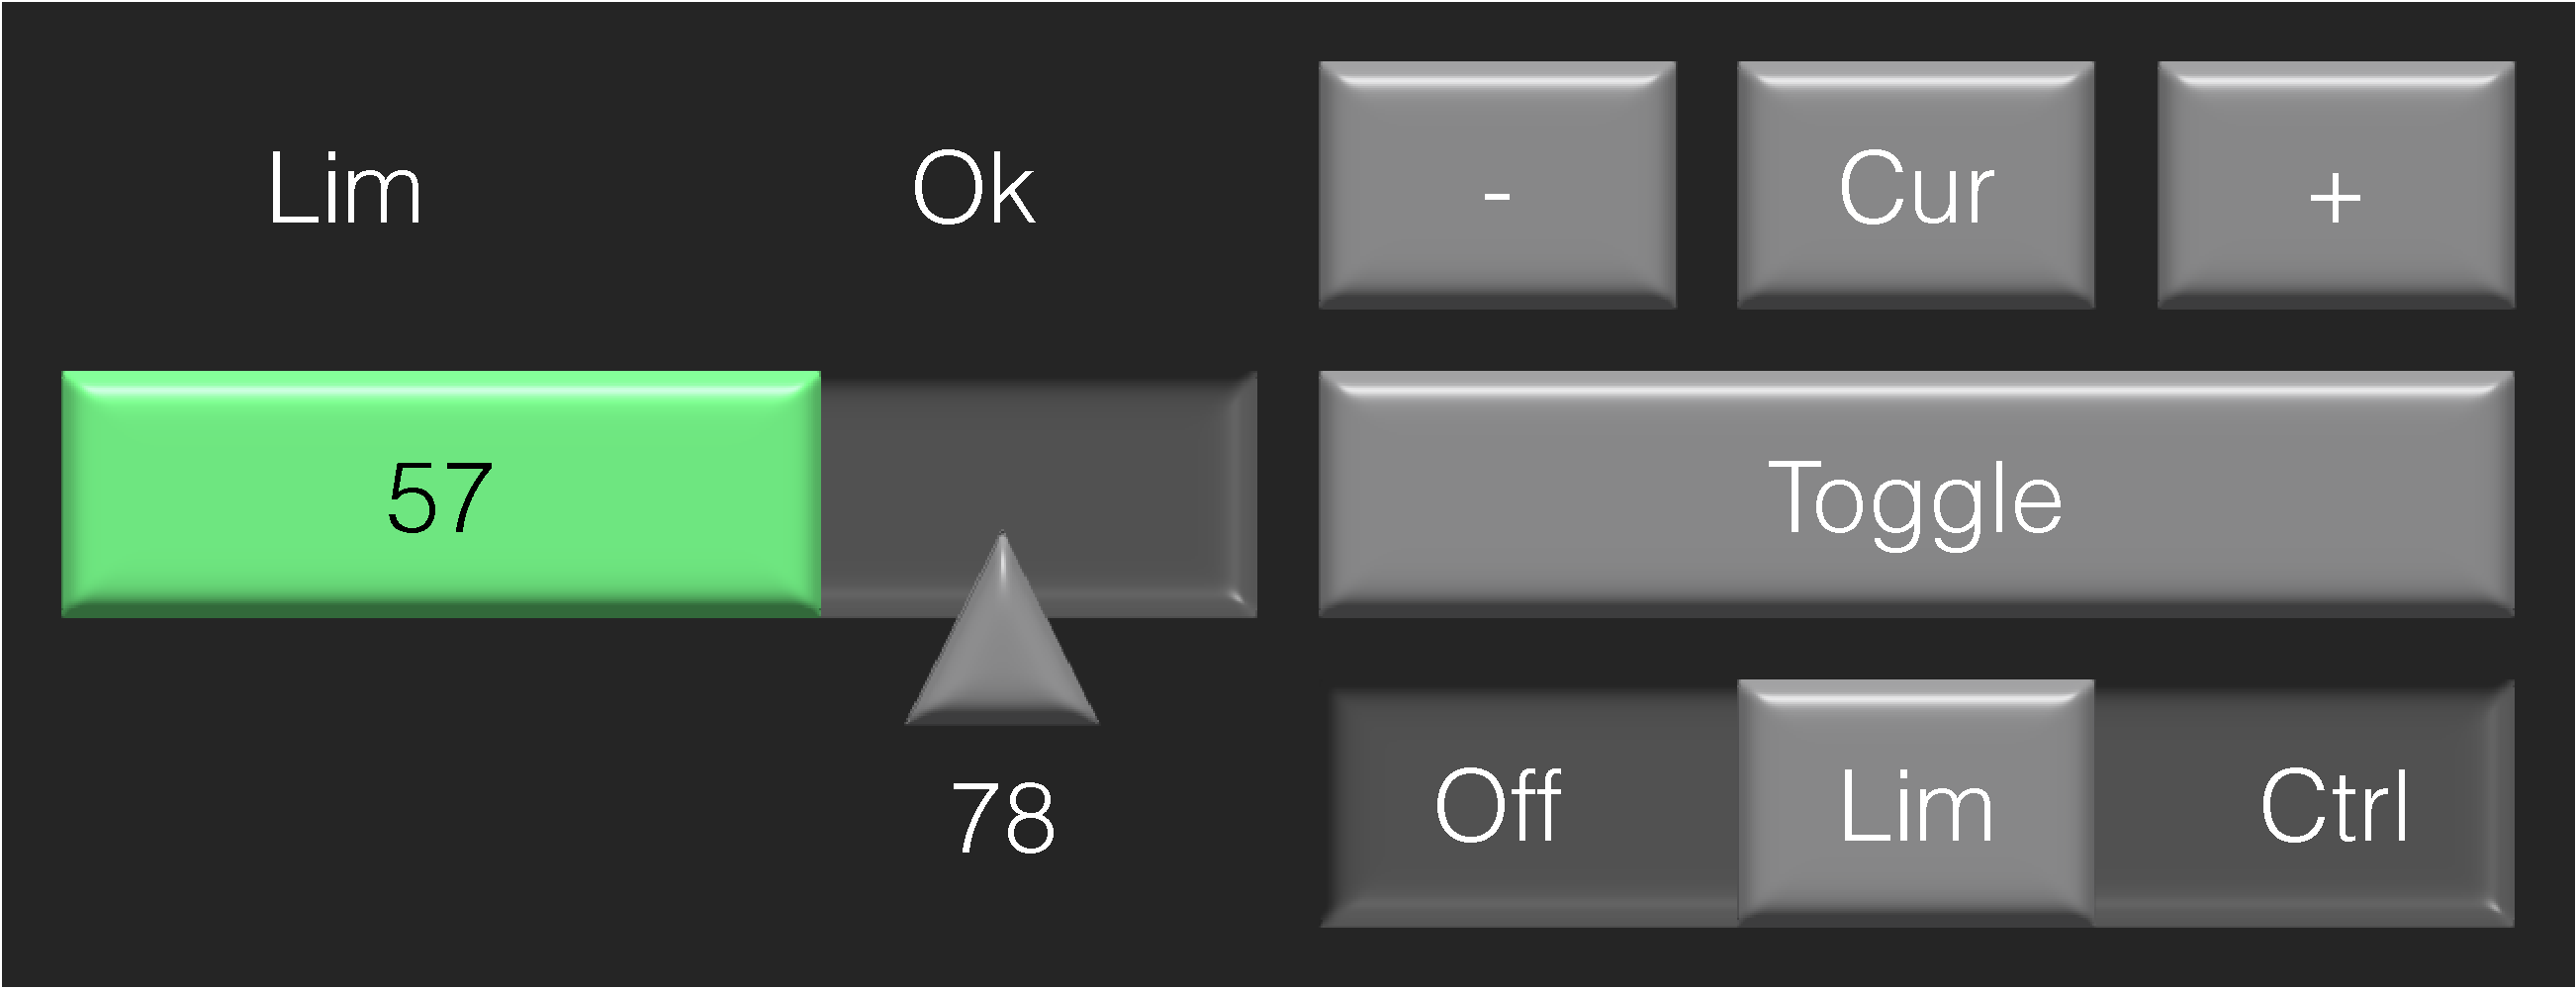
\includegraphics[width=\columnwidth,page=1]{drawings.pdf}
\end{center}
\caption{A mockup of the example GUI}
\label{fig-gui-example}
\end{figure}

\clearpage

\begin{lstlisting}[caption=Interface of the speed controller]
interface 
	SpeedController
is
	{
		system: {
			desiredMode:	text out,
			desiredSpeed:	number out,
			actualMode:		text in,
			actualSpeed:	number in
		},
		user: {
			mode:	Label,
			status:	Label,
			actual:	Gauge,
			desired:	Slider,
			increment:	Button,
			decrement:	Button,
			current:	Button,
			toggle:	Button,
			switch:	SegmentedSwitch
		}
	}
\end{lstlisting}

\clearpage

\begin{lstlisting}[caption=The speed controller interaction]
interaction 
	(TheSpeedController)
implementing
	SpeedController
is
	(bind ({
		system:{
			desiredMode: (theDesiredMode),
			desiredSpeed: (theDesiredSpeed),
			actualMode: (theActualMode),
			actualSpeed: (theActualSpeed)          
		},
		user:{	
			mode: (Label (active) 
				with value (theActualMode)),	
			status: (Label (active) 
				with value (
					if ((theActualMode) != (theDesiredMode))
					then ("Wrong mode")
					else if (((theDesiredMode) != ("Off")) 
					and((theActualSpeed)>(theDesiredSpeed)))
					then ("Over speed")
					else ("Ok")
				)),
			actual: (Gauge (active) 
				with value (theActualSpeed)),
			desired: (Slider (active) 
				with value (theDesiredSpeed)
				selecting (new(theDesiredSpeed))),
			increment: (Button (active) 
				with text ("+")
				triggering ( (new(theDesiredSpeed)) = 
				((previous(theDesiredSpeed))+(5)))),
			decrement: (Button (active) 
				with text ("-")
				triggering ( (new(theDesiredSpeed)) = 
				((previous(theDesiredSpeed))-(5)))),
			current: (Button (active) 
				with text ("Cur")
				triggering ( (new(theDesiredSpeed)) = 
				(round (theActualSpeed) to (5)))),
			toggle: (Button (active) 
				with text ("Toggle")
				triggering ( (new(theDesiredMode))=(
					if((previous(theDesiredMode))==("Off"))
					then(theSelectedMode)
					else("Off")
				))),
			switch: (SegmentedSwitch (active) 
				with choices (["Off","Lim","Ctrl"]) 
				selecting (theSelectedMode))
		}
	}) : (all
		(make (theDesiredSpeed) flow)  
		(make (theDesiredMode) flow) 
	))
\end{lstlisting}


\clearpage

\begin{lstlisting}[caption=The speed controller interaction unfolded]
interaction 
	(TheSpeedController)
implementing
	SpeedController
is
	(bind ({
		system:{
			desiredMode: (theDesiredMode),
			desiredSpeed: (theDesiredSpeed),
			actualMode: (theActualMode),
			actualSpeed: (theActualSpeed)          
		},
		user:{	
			mode: 	
				(bind(x1) : 
					((all
						((x1.value)=(theActualMode))
					)=(active))),
			status: 
				(bind(x2) : 
					((all((x2.value)=(if ((theActualMode) != (theDesiredMode))
						then ("Wrong mode")
						else if (((theDesiredMode) != ("Off")) and((theActualSpeed)>(theDesiredSpeed)))
						then ("Over speed")
						else ("Ok")))
					)=(active))),
			actual: 
				(bind(x3) : 
					((all
						((x3.value)=(theActualSpeed))
					)=(active))),
			desired:
				(bind(x4) : (
					(all
						((x4.value)=(theDesiredSpeed))
						((new(theDesiredSpeed))=(x4.selection))
					)=(active))),
			increment: 
				(bind(x5) : (
					(all((x5.value)=("+"))(((new(theDesiredSpeed))=((previous(theDesiredSpeed))+(5)))=(x5.click)))=(active))),
			decrement: 
				(bind(x6) : (
					(all((x6.value)=("-"))(((new(theDesiredSpeed))=((previous(theDesiredSpeed))-(5)))=(x6.click)))=(active))),
			current: 
				(bind(x7) : (
					(all((x7.value)=("Cur"))(((new(theDesiredSpeed))=(round (theActualSpeed) to (5)))=(x7.click)))=(active))),
			toggle: 
				(bind(x8) : (
					(all((x8.value)=("Toggle"))(
					( (new(theDesiredMode))=(
						if((previous(theDesiredMode))==("Off"))
						then(theSelectedMode)
						else("Off")
					))=(x8.click)))=(active))),
			switch: 
				(bind(x9) : ((all
					((x9.choices)=(["Off","Lim","Ctrl"]))
					((theSelectedMode)=((["Off","Lim","Ctrl"])[(x9.selection)])))=(active))),		
		}
	}) : (all
		((theDesiredSpeed) = 
			(if ((new(theDesiredSpeed)) is active) 
			then (new(theDesiredSpeed)) 
			else (previous(theDesiredSpeed))))
		((theDesiredMode) = 
			(if ((new(theDesiredMode)) is active) 
			then (new(theDesiredMode)) 
			else (previous(theDesiredMode))))
	))
\end{lstlisting}

Once totally unfolded, the SpeedController uses the following base interactions :

\begin{itemize}
	\item \code{bind\$:\$}
	\item \code{\$=\$}
	\item \code{all\$\$}
	\item \code{if\$then\$else\$}
	\item \code{previous\$}
	\item \code{\$+\$}
	\item \code{\$-\$}
	\item \code{\$==\$}
	\item \code{\$and\$}
	\item \code{round\$to\$}
	\item \code{\{system:\{desiredMode:\$,desiredSpeed:\$...\},user:\{...\}\}}
	\item \code{5}
	\item \code{active}
	\item \code{"Wrong Mode"}
	\item Other constants...
\end{itemize}


\clearpage


\section{Assessment}

We provide an assessment of the description capabilities of the defined language. 

\begin{itemize}
\item Flows : continuous
\item Events : discrete
\item composition of flows and events to build behaviors
\end{itemize}
These notions are embedded in a reusable component implementing the notion of interactor. 


Give a positionning with respect to the requirements


\section{Harnessing  LIDL }

\begin{itemize}

\item Verification 
\item Code generation 
\item Test and automatic test generation

\end{itemize}


Give a positionning with respect to the requirements



\section{Related work}

\begin{itemize}
\item Notion of interactor: York, 
\item Extended LUSTRE et lien avec le langage Lustre
\end{itemize}
None of the previous approaches handle 

%ARRIVER à UN TABLEAU COMPARATIF




\section{Conclusion and future work}

\begin{itemize}
\item  A language for concurent interface design among different stakeholders, programming, verifying, testing
\item Code generation
\item prototype

\end{itemize}
Future  work
\begin{itemize}
\item Tool support 
\item Handling the description and the verification of a whole system including the human. We believe that the integration of the human is eased by the abstraction level in which LIDL components are described [CITER RUSHBY]
\item Verification of other properties, Honesty, freshness, device overload 
\item temporal properties related to delays and their impact on the architecture of the interface
 
\end{itemize}

\subsection{TO DO list}

\begin{itemize}



\item yamine
\begin {itemize}
\item Choisir une figure pour l'étude de cas parmi les 10 choix donnés
\end {itemize}


\item bruno

\item vincent
\begin{itemize}
\item \sout{renommage pour éviter homonymie}
\item \sout{supprimer les bind, this, all}
\item exprimer les basic constructs
\item éviter les éléments inachevés
\item \sout{flow pourrait devenir flow\_mk}
\item  \sout{changer figure étude de cas.}
\end{itemize}



\end{itemize}


\appendix

\section{Appendix}



\subsection{Generic}

Some generic interactions are necessary to make the language useful. Listing~\ref{lst:generic} shows the most important ones.

\begin{lstlisting}[caption=Section of the standard LIDL library regarding generic interactions,label={lst:generic}]
// (if(cond)then(a)else(b)) is similar 
// to the ternary operator cond?a:b in C
interaction
	(if (condition:boolean in)
	then (a:<type>)
	else (b:<type>))
implementing
	-<type>
is
	`native`
	
// ((a) is active) projects (a) into the 
// activation type. It removes the value of 
// (a), only keeping its activation
interaction
	((a:<type> in) is active)
implementing
	activation out
is
	`native`

// ((a) is true) takes a boolean and returns
// an activation which is active if and only
// if (a) is active and true
interaction
	((a:boolean in) is true)
implementing
	activation out
is
	`native`

// (bind(a):(b)) is equivalent to (a), 
// but it also execute the behavior (b) 
// in parallel. (b) can have an effect 
// on (a) by using variables
interaction
	(bind (a:<type> data) : (b:activation out))
implementing
	<type> data
is
	`native`

interaction 
	((a: <type> in) default (b: <type> in))
implementing
	<type> out
is
	(if ((a) is active) then (a) else (b))
\end{lstlisting}

\subsection{Lists}


\begin{lstlisting}[caption=Section of the standard LIDL library regarding lists interactions,label={lst:lists}]
// Get list element
interaction 
	( (a:[<type>]in) [ (index:number in) ] )
implementing
	<type> out
is
	`native`
	
// Set list element
interaction 
	( (a:[<type>]out) [ (index:number in) ] )
implementing
	<type> in
is
	`native`
	
// Compose list
interaction
	([(first:<type>in),(second:<type>in),...,(last:<type>in)])
implementing
	<type> out
is
	`native`
	
	
// Decompose list
interaction
	([(first:<type>out),(second:<type>out),...,(last:<type>out)])
implementing
	<type> in
is
	`native`
\end{lstlisting}



\subsection{Behavior}
What is a behavior ? Very generally, a behavior is some kind of action that is executed at some points in time. This is why we define the \lstinline{Behavior} interface to be equivalent to the \lstinline{activation in} interface. This means that interactions implementing the \lstinline{Behavior} interface receive a flow of \lstinline{activation}. When they receive the \lstinline{active} value, they are effective, when they receive the \lstinline{inactive} value, they are not effective. 

The LIDL standard library defines some useful basic behaviors, as shown on Listing~\ref{lst:behavior}.

\begin{lstlisting}[caption=Section of the standard LIDL library regarding Behaviors,label={lst:behavior}]
interface 
	Behavior 
is
	activation in

interaction 
	((a:<type>out) = (b:<type>in))
implementing
	Behavior
is 
	`native`

interaction 
	(all (a:activation out) (b:activation out))
implementing 
	Behavior
is
	`native`
	
interaction 
	(either (a:activation out) (b:activation out))
implementing 
	Behavior
is
	`native`
	
interaction 
	(always (a:activation out))
implementing 
	Behavior
is
	`native`
	
interaction
	(when (condition:activation in) : (effect:activation out) )
implementing
	Behavior
is
	((effect)=(condition))

interaction 
	(make (a: <type> s) flow)
implementing
	Behavior
is
	((a) = ((new(a)) default (previous(a))))
  
\end{lstlisting}


\subsection{Activation}


\begin{lstlisting}
interaction
	(active)
implementing
	activation out
is
	`native`
\end{lstlisting}



\subsection{Boolean operators}

What is a boolean operator ? Very generally, it is something that takes some parameters and returns a boolean. This is why we define de \lstinline{Boolean} interface to be equivalent to the \lstinline{boolean out} interface. This means that interactions implementing the \lstinline{Boolean} interface return a flow of \lstinline{boolean} which depends on their parameters.

The LIDL standard library defines some useful basic boolean operators, as shown on Listing~\ref{lst:boolean}.

\begin{lstlisting}[caption=The Number expressions definitions of the standard LIDL library,label={lst:boolean}]
interface 
	Boolean 
is
	boolean out

interaction 
	(not (a:boolean in))
implementing 
	Boolean
is
	`native`

interaction 
	((a:boolean in) and (b:boolean in))
implementing 
	Boolean
is
	`native`
	
interaction 
	((a:boolean in) or (b:boolean in))
implementing 
	Boolean
is
	(not((not(a))and(not(b))))
	
interaction 
	((a:boolean in) xor (b:boolean in))
implementing 
	Boolean
is
	(((a)or(b))and(not((a)and(b))))
	
interaction 
	((a:boolean in) nand (b:boolean in))
implementing 
	Boolean
is
	(not((a)and(b))
	
interaction	
	((a:boolean in) nor (b:boolean in))
implementing 
	Boolean
is
	(not((a)or(b))

interaction 
	((a:boolean in) implies (b:boolean in))
implementing 
	Boolean
is
	(not((a)and(not(b))))
	
interaction 
	((a:boolean in) is equivalent to (b:boolean in))
implementing 
	Boolean
is
	(not((a)xor(b)))
	
interaction 
	((a:boolean in) inhibited by (b:boolean in))
implementing 
	Boolean
is
	((a)and(not(b)))
	
interaction 
	((a:<type>in) == (b:<type>in))
implementing
	Boolean
is 
	`native`
	
interaction 
	((a:<type>in) != (b:<type>in))
implementing
	Boolean
is 
	(not((a)==(b)))

\end{lstlisting}


\subsection{Numeric operators}

What is a numeric operator ? Very generally, it is something that takes some parameters and returns a number. This is why we define de \lstinline{Numeric} interface to be equivalent to the \lstinline{number out} interface. This means that interactions implementing the \lstinline{Numeric} interface return a flow of \lstinline{number} which depends on their parameters.

The LIDL standard library defines some useful basic numeric operators, as shown on Listing~\ref{lst:numeric}.

\begin{lstlisting}[caption=The Number expressions definitions of the standard LIDL library,label={lst:numeric}]
interface 
	Numeric 
is
	number out

// opposite
interaction 
	(- (a:number in))
implementing 
	Numeric
is
	`native`

// sum
interaction 
	((a:number in) + (b:number in))
implementing 
	Numeric
is
	`native`
	
// difference
interaction 
	((a:number in) - (b:number in))
implementing 
	Numeric
is
	((a)+(-(b)))

// inverse
interaction
	(inverse (a:number in))
implementing
	Numeric
is
	`native`

// multiplication
interaction 
	((a:number in) * (b:number in))
implementing 
	Numeric
is
	`native`

// division
interaction 
	((a:number in) / (b:number in))
implementing 
	Numeric
is
	((a)*(inverse(b)))
\end{lstlisting}





\subsection{Widgets}

The LIDL standard library defines some widgets, as shown on Listing~\ref{lst:widgets}.

\begin{lstlisting}[caption=A standard widget library,label={lst:widgets}]
////////////////////////////////////////////////
interface
	Label
is
	{
		value : text out
	}

interaction 
	(Label (status: activation in)
	with title (theTitle: text in))
implementing
	Label
is
	(bind(this) : (when (status) : (all
			((this.value)=(theTitle)))
	)))

////////////////////////////////////////////////
interface 
	Gauge
is
	{
		value : number out
	}

interaction 
	(Gauge (status: activation in)
 	with value (theValue: number in))
implementing 
	Gauge
is
	(bind(this) : (when (status) : (all
		((this.value)=(theValue))
	)))
	
////////////////////////////////////////////////
interface 
	Button
is
	{
		value: text out,
		click : activation in	
	}

interaction 
	(Button (status: activation in) 
	with title (theTitle: text in) 
	trigerring (onClick: activation out))
implementing
	Button
is
	(bind(this) : (when (status) : (all
			((this.value)=(theTitle))
			((onClick)=(this.click))
	)))
	
	
    
////////////////////////////////////////////////
interface 	
	SegmentedSwitch
is
	{
		choices : [text] out,
		selection : number in
	}

interaction 
	(SegmentedSwitch (status: activation in) 
	with choices (theChoices: [text] in)
	selecting (theSelection: text out))
implementing
	SegmentedSwitch
is
	(bind(this) : (when (status) : (all
			((this.choices)=(theChoices))
			((theSelection)=
				((theChoices)[(this.selection)]))
	)))
	
////////////////////////////////////////////////
interface 
	Slider
is
	{
		value : number out
		selection : number in,
	}

interaction 
	(Slider (status: activation in)
	with value (theValue: number in)
	selecting (theSelection: number out))
implementing
	Slider
is
	(bind(this) : (when (status) : (all
			((this.value)=(theValue))
			((theSelection)=(this.selection))
	)))


////////////////////////////////////////////////

\end{lstlisting}


Here we put the LIDL source code of the case study and probably the promela code and Event-B code etc. 



\acks

Acknowledgments, if needed.

% We recommend abbrvnat bibliography style.

\bibliographystyle{abbrvnat}

% The bibliography should be embedded for final submission.

\begin{thebibliography}{}
\softraggedright
\bibitem{bea} 
  Bureau d'Enqu\^etes et d'Analyses pour la s\'ecurit\'e de l'Aviation Civile. 
  Rapport du Vol AF 447 du 1$^{er}$ Juin 2009.
  http://www.bea.aero/fr/enquetes/vol.af.447/rapport.final.fr.php.
\bibitem{DO178C}
  DO178C. 
  Software Considerations in Airborn Systems and Equipment
  Certification, release C.
  2012.
  RTCA,Inc.
\bibitem{ARINC}
  ARINC 661.
  Cockpit Display Systems Interfaces to User Systems.
  http://www.aviation-ia.com/aeec/projects/cds/index.html.
  Airlines Electronic Engineering Committee.
\bibitem{scade-display}
  http://www.esterel-technologies.com/products/scade-display.

%\bibitem[Smith et~al.(2009)Smith, Jones]{smith02}
%P. Q. Smith, and X. Y. Jones. ...reference text...

\end{thebibliography}


\end{document}

%                       Revision History
%                       -------- -------
%  Date         Person  Ver.    Change
%  ----         ------  ----    ------

%  2013.06.29   TU      0.1--4  comments on permission/copyright notices

